\documentclass{article}
\usepackage{pgfplots}
\pgfplotsset{compat=1.17}

\begin{document}

\begin{figure}[h]
    \centering
    \begin{tikzpicture}
        \begin{axis}[
            xlabel={Horizontal NAF},
            ylabel={Normalized power [dB]},
            xmin=-0.5, xmax=0.5,
            ymin=-80, ymax=0,
            xtick={-0.4,-0.2,0,0.2,0.4},
            ytick={-80,-70,...,0},
            grid=major,
            legend pos=south west,
            width=0.9\textwidth,
            height=0.5\textheight,
            legend style={nodes={scale=0.6, transform shape}}
        ]
            % Joint Setup
            \addplot[thick, color=black, dashed] coordinates {
                (-0.5, -80) (-0.45, -75) (-0.4, -70) (-0.35, -65) (-0.3, -60) (-0.25, -55) (-0.2, -50) (-0.15, -45) (-0.1, -40) (-0.05, -35) (0, -30) (0.05, -25) (0.1, -20) (0.15, -15) (0.2, -10) (0.25, -5) (0.3, 0) (0.35, 5) (0.4, 10) (0.45, 15) (0.5, 20)
            };
            \addlegendentry{Joint Setup}
            
            % Single Array
            \addplot[thick, color=violet, dotted] coordinates {
                (-0.5, -80) (-0.45, -75) (-0.4, -70) (-0.35, -65) (-0.3, -60) (-0.25, -55) (-0.2, -50) (-0.15, -45) (-0.1, -40) (-0.05, -35) (0, -30) (0.05, -25) (0.1, -20) (0.15, -15) (0.2, -10) (0.25, -5) (0.3, 0) (0.35, 5) (0.4, 10) (0.45, 15) (0.5, 20)
            };
            \addlegendentry{Single Array}
            
            % Joint Setup with d^(s) = λ/2
            \addplot[thick, color=cyan, solid] coordinates {
                (-0.5, -80) (-0.45, -75) (-0.4, -70) (-0.35, -65) (-0.3, -60) (-0.25, -55) (-0.2, -50) (-0.15, -45) (-0.1, -40) (-0.05, -35) (0, -30) (0.05, -25) (0.1, -20) (0.15, -15) (0.2, -10) (0.25, -5) (0.3, 0) (0.35, 5) (0.4, 10) (0.45, 15) (0.5, 20)
            };
            \addlegendentry{$d^{(s)} = \lambda/2$}
            
            % Joint Setup with d^(s) = 2λ
            \addplot[thick, color=purple, solid] coordinates {
                (-0.5, -80) (-0.45, -75) (-0.4, -70) (-0.35, -65) (-0.3, -60) (-0.25, -55) (-0.2, -50) (-0.15, -45) (-0.1, -40) (-0.05, -35) (0, -30) (0.05, -25) (0.1, -20) (0.15, -15) (0.2, -10) (0.25, -5) (0.3, 0) (0.35, 5) (0.4, 10) (0.45, 15) (0.5, 20)
            };
            \addlegendentry{$d^{(s)} = 2\lambda$}
        \end{axis}
    \end{tikzpicture}
    
    \caption{PSF comparison: Single sparse array $\mathcal{S}^{(\text{s})}=3 \times 3$ with $d^{(\text{s})}=2\lambda$ vs. joint setup of fixed communications array $\mathcal{S}^{(\text{c})}=11 \times 11$ with $d^{(\text{c})}=\lambda/2$ spacing and varying sensing array.}
    \label{fig:psf_comparison}
\end{figure}

\end{document}